\section{Ejercicio 7}
Para entender el schedler, hemos corrido  una serie de task .

\begin{figure}[ht]
	\begin{center}
		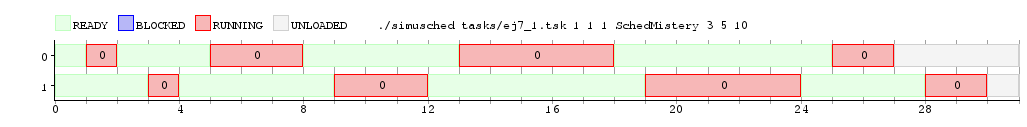
\includegraphics[width=1\columnwidth]{imagenes/ej7_1.png}
		\caption{Dos \texttt{TaskCPU} con 20 quantums.}
	\end{center}
\end{figure}

Hemos Corrido 3 tasks, cada una con 20 quantums, sin ninguna interupción. Se puede apreciar que una vez acabadosus quantums, es agregado en la siguiente cola con menor prioridad , si hay , y una vez desencolado los task pendientes en una cola pasa a la siguiente.


\begin{figure}[ht]
	\begin{center}
		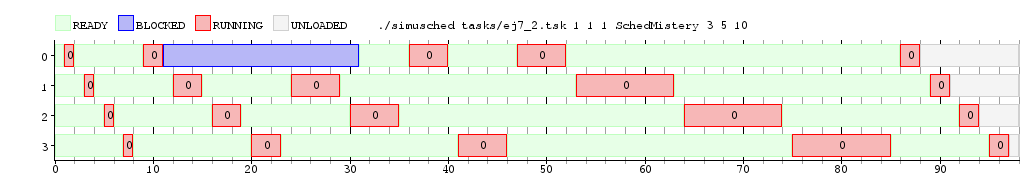
\includegraphics[width=1\columnwidth]{imagenes/ej7_2.png}
		\caption{\texttt{TaskBatch} corriendo con $\texttt{total\_cpu} = 4$,
		$\texttt{cant\_bloqueos} = 2$.}
	\end{center}
\end{figure}

Hemos Corrido 3 tasks, una con 20 quantums, sin ninguna interupción, y otras dos que por cada 2 quantums se bloquea 1 . Como se puede apreciar este schedler permite starvation, haciendo que la tareas con pocas interupciones se acumulen en las colas con menor prioridad, esperando que las tasks de mayor prioridad acaben para que les toque a ellos.
